% CVPR 2022 Paper Template
% based on the CVPR template provided by Ming-Ming Cheng (https://github.com/MCG-NKU/CVPR_Template)
% modified and extended by Stefan Roth (stefan.roth@NOSPAMtu-darmstadt.de)

\documentclass[10pt,twocolumn,letterpaper]{article}

%%%%%%%%% PAPER TYPE  - PLEASE UPDATE FOR FINAL VERSION
% \usepackage[review]{cvpr}      % To produce the REVIEW version
% \usepackage{cvpr}              % To produce the CAMERA-READY version
\usepackage[pagenumbers]{cvpr} % To force page numbers, e.g. for an arXiv version

% Include other packages here, before hyperref.
\usepackage{graphicx}
\usepackage{amsmath}
\usepackage{amssymb}
\usepackage{booktabs}

% It is strongly recommended to use hyperref, especially for the review version.
% hyperref with option pagebackref eases the reviewers' job.
% Please disable hyperref *only* if you encounter grave issues, e.g. with the
% file validation for the camera-ready version.
%
% If you comment hyperref and then uncomment it, you should delete
% ReviewTempalte.aux before re-running LaTeX.
% (Or just hit 'q' on the first LaTeX run, let it finish, and you
%  should be clear).
\usepackage[pagebackref,breaklinks,colorlinks]{hyperref}


% Support for easy cross-referencing
\usepackage[capitalize]{cleveref}
\crefname{section}{Sec.}{Secs.}
\Crefname{section}{Section}{Sections}
\Crefname{table}{Table}{Tables}
\crefname{table}{Tab.}{Tabs.}


%%%%%%%%% PAPER ID  - PLEASE UPDATE
\def\cvprPaperID{0}
\def\confName{CSE 559a}
\def\confYear{\the\year{}}


\begin{document}

%%%%%%%%% TITLE - PLEASE UPDATE
\title{Progress Report: AutoVision --- Learning to Automatically Design Vision Pipelines for Classification and Segmentation}

\author{
Yusheng Tan \hspace{1in} Yuanjun Feng \hspace{1in} Yimu Liu
}
\maketitle

%%%%%%%%% ABSTRACT
\begin{abstract}
We present a progress report for AutoVision, a project that explores whether an AI coding agent can autonomously improve computer vision pipelines through iterative code modification and evaluation. Building on the AutoResearch framework~\cite{Karpathy2025AutoResearch, Erhard2025AutoResearchCIFAR}, our system uses a large language model (Claude) to iteratively modify training scripts, evaluating each modification under a fixed five-minute compute budget and retaining only those changes that yield measurable improvement. We apply this methodology to two complementary vision tasks: image classification on CIFAR-10~\cite{Krizhevsky2009CIFAR} using a ResNet-20~\cite{He2016ResNet} baseline, and semantic segmentation on the Oxford-IIIT Pet dataset~\cite{Parkhi2012Pets} using a U-Net~\cite{Ronneberger2015UNet} baseline. In this report, we describe our current progress: we have collected and validated both datasets, adopted and tested the ResNet-20 classification baseline from the Erhard repository, and studied the agent loop infrastructure. We outline our detailed approach and the remaining steps toward our final evaluation.
\end{abstract}

%%%%%%%%% BODY TEXT
\section{Project Overview}

Our project investigates whether an AI coding agent can serve as a principled replacement for the manual hyperparameter tuning and architecture search process that is central to building competitive vision models. The key insight, drawn from the AutoResearch framework~\cite{Karpathy2025AutoResearch}, is to frame the search process as an iterative agent loop: an LLM-based coding agent reads a training script and a natural-language instruction file, proposes a single modification, and the modification is evaluated under a strict five-minute wall-clock budget. Modifications that improve the validation metric are retained; all others are reverted.

We apply this approach to two tasks:
\begin{enumerate}
    \item \textbf{Image Classification}: CIFAR-10 with a ResNet-20 baseline~\cite{He2016ResNet}. The ResNet-20 architecture was specifically designed for CIFAR-scale images and provides a well-understood starting point, typically achieving $\sim$91--92\% test accuracy with standard training.
    \item \textbf{Semantic Segmentation}: Oxford-IIIT Pet dataset~\cite{Parkhi2012Pets} with a U-Net baseline~\cite{Ronneberger2015UNet}. This task extends our investigation to a dense prediction setting, where the agent must optimize for pixel-level accuracy (mIoU, Dice coefficient) rather than global classification accuracy.
\end{enumerate}

\noindent\textbf{Changes from Proposal.} Our project goals and methodology remain unchanged from the original proposal. We continue to target both the minimum goal (successful agent loop for classification) and the maximum goal (both tasks with cross-task analysis of agent behavior).


\section{Team Member Roles/Tasks}
\label{sec:roles}

\subsection{Yusheng Tan}

\begin{enumerate}

\item Implement and maintain the AutoResearch outer loop, including the agent harness, timing mechanism, and keep/revert logic.
\item Author and refine the \texttt{program.md} instruction files for both the classification and segmentation experiments.
\item Coordinate the overall experimental workflow, maintain logs of agent decisions across runs, and manage the shared codebase.

\end{enumerate}

\subsection{Yuanjun Feng}

\begin{enumerate}

\item Implement and validate the ResNet-20 classification baseline on CIFAR-10, following the original He~\etal~\cite{He2016ResNet} specification.
\item Run the agent loop for the classification task and record all experimental outcomes.
\item Summarize and analyze the sequence of modifications the agent made throughout the classification search.

\end{enumerate}

\subsection{Yimu Liu}

\begin{enumerate}

\item Implement the U-Net segmentation baseline on the Oxford-IIIT Pet dataset with a pretrained ResNet encoder.
\item Run the agent loop for the segmentation task and record results.
\item Implement evaluation metrics (mIoU, Dice coefficient) and produce comparative plots for the final report.

\end{enumerate}

\section{Collaboration Strategy}

Our team uses a shared GitHub repository for version control, with each member working on a dedicated branch corresponding to their component (classification baseline, segmentation baseline, and AutoResearch loop). We merge changes to the main branch through pull requests after code review. Data and model checkpoints are stored on a shared Google Drive accessible to all members. We hold brief synchronous meetings twice per week via Zoom to discuss progress and coordinate next steps, and maintain an active group chat for asynchronous communication.

\section{Proposed Approach}

Our approach consists of three interconnected components, described below.

\subsection{Baseline Models}

\textbf{Classification.} For the classification baseline, we adopt the ResNet-20 implementation from the \texttt{autoresearch-cifar10} repository~\cite{Erhard2025AutoResearchCIFAR}, which provides a faithful reproduction of the architecture described in He~\etal~\cite{He2016ResNet} (Section~4.2). The model consists of three groups of residual blocks ($n=3$, totaling $6n+2=20$ layers) with filter widths 16$\to$32$\to$64, identity shortcuts with zero-padding (Option~A from the original paper), and Kaiming initialization. Training uses SGD with momentum~0.9, weight decay~$10^{-4}$, initial learning rate~0.1 with step-based decay (divided by~10 at steps 32k and 48k out of 64k total), batch size~128, and standard CIFAR augmentations (4-pixel padding with random 32$\times$32 crop, random horizontal flip). This baseline achieves 91.89\% test accuracy in a full run~\cite{Erhard2025AutoResearchCIFAR}, consistent with the published result of 91.25\%.

\textbf{Segmentation.} For the segmentation baseline, we implement U-Net~\cite{Ronneberger2015UNet} using a pretrained ResNet-34 encoder (from \texttt{torchvision.models}) as the contracting path, with a symmetric expanding path using transposed convolutions and skip connections. The segmentation target is a 3-class trimap (foreground, background, boundary) from the Oxford-IIIT Pet dataset. We train with cross-entropy loss and evaluate using mean Intersection over Union (mIoU) and Dice coefficient. We are also aware of DeepLabV3+~\cite{Chen2018DeepLabV3} as a potentially stronger baseline and may explore it depending on the agent's modifications.

\subsection{AutoResearch Agent Loop}

Following the AutoResearch paradigm~\cite{Karpathy2025AutoResearch, Erhard2025AutoResearchCIFAR}, we do not implement a separate outer-loop script. Instead, the agent (Claude, via Claude Code) is given a \texttt{program.md} file containing detailed instructions and operates autonomously. The loop proceeds as follows:

\begin{enumerate}
    \item The agent reads \texttt{program.md} and the current \texttt{train.py}, which is the \emph{only} file it may modify.
    \item The agent proposes a single modification, edits \texttt{train.py}, and commits the change via \texttt{git}.
    \item The agent runs the training script under a fixed wall-clock time budget (5~minutes for classification). Output is redirected to a log file to avoid flooding the agent's context.
    \item If \texttt{best\_test\_acc} improves, the commit is kept and the git branch advances. If it does not improve, the agent performs a \texttt{git reset} to revert to the previous best state.
    \item The agent appends each result (commit hash, accuracy, memory usage, keep/discard status, description) to a \texttt{results.tsv} log file.
    \item The process repeats indefinitely until manually stopped, typically running 50--100+ iterations overnight.
\end{enumerate}

The \texttt{program.md} file also encodes constraints (e.g., \texttt{prepare.py} is read-only, no new dependencies) and a simplicity criterion: changes that add complexity must justify it with significant accuracy gains.

\subsection{Analysis}

After completing the agent loops for both tasks, we will analyze: (1)~the trajectory of accuracy/mIoU improvement over iterations; (2)~the categories of modifications the agent favors (e.g., data augmentation, architecture changes, optimizer tuning, regularization); and (3)~whether the agent's strategies differ meaningfully between classification and segmentation.


\section{Data}

\subsection{CIFAR-10}

CIFAR-10~\cite{Krizhevsky2009CIFAR} consists of 60,000 color images of size $32\times32$ across 10 mutually exclusive categories: airplane, automobile, bird, cat, deer, dog, frog, horse, ship, and truck. The dataset is split into 50,000 training images and 10,000 test images. It is available through \texttt{torchvision.datasets.CIFAR10} and requires no manual preprocessing. We have downloaded and verified the dataset. \cref{fig:cifar10} shows representative samples from each class.

\begin{figure}[t]
    \centering
    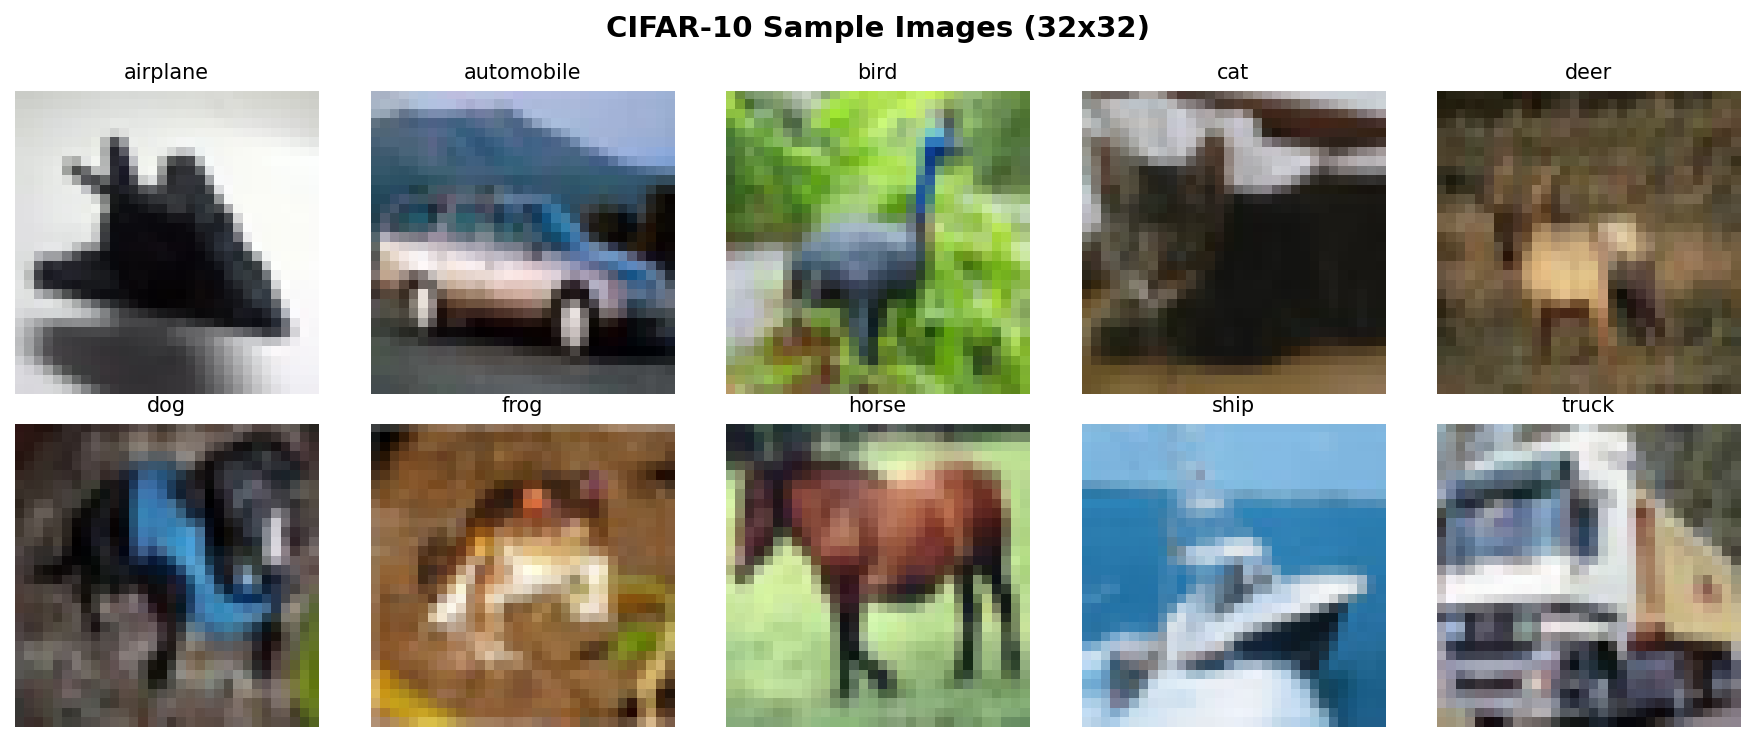
\includegraphics[width=\linewidth]{figures/cifar10_samples.png}
    \caption{Sample images from the CIFAR-10 dataset, showing the characteristic $32\times32$ resolution across representative categories.}
    \label{fig:cifar10}
\end{figure}

\subsection{Oxford-IIIT Pet}

The Oxford-IIIT Pet dataset~\cite{Parkhi2012Pets} contains 7,349 images of cats and dogs spanning 37 breed categories. Each image is accompanied by a pixel-level trimap annotation with three classes: foreground (pet), background, and boundary. The training/validation split contains 3,680 images and the test split contains 3,669 images. Images vary in resolution and are resized to $256\times256$ for training. The dataset is available through \texttt{torchvision.datasets.OxfordIIITPet}. We have downloaded the dataset and confirmed that the segmentation masks load correctly. \cref{fig:pet} illustrates example images with their associated trimap annotations.

\begin{figure}[t]
    \centering
    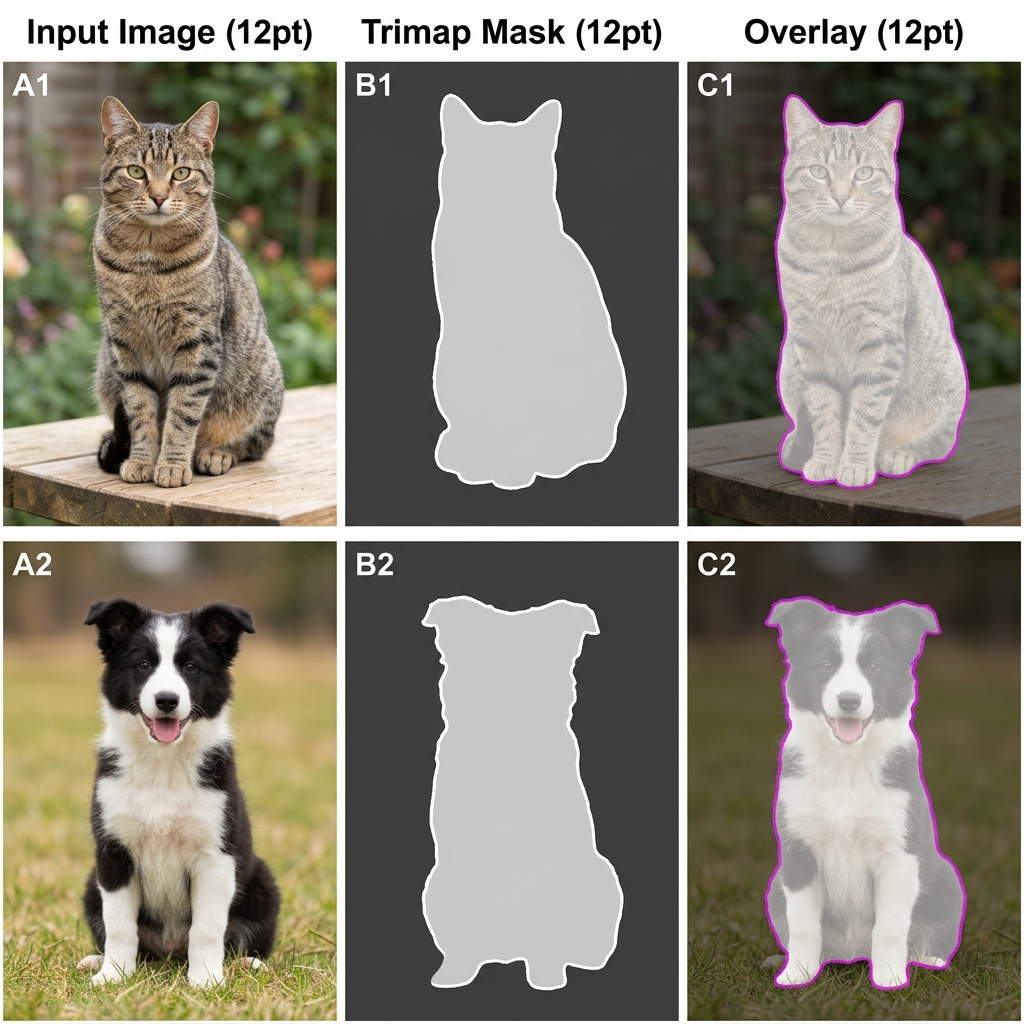
\includegraphics[width=\linewidth]{figures/pet_samples.png}
    \caption{Sample images from the Oxford-IIIT Pet dataset with corresponding trimap segmentation masks. The trimaps distinguish foreground (pet), background, and boundary regions.}
    \label{fig:pet}
\end{figure}


\section{Initial Results}

We have completed the following steps toward our project goals:

\begin{enumerate}
    \item \textbf{Data collection and verification.} Both CIFAR-10 and the Oxford-IIIT Pet dataset have been downloaded via \texttt{torchvision}, loaded into PyTorch dataloaders, and visually inspected to confirm correct labeling and mask alignment (see \cref{fig:cifar10,fig:pet}).

    \item \textbf{Reference codebase study.} We have cloned and studied both the original AutoResearch repository by Karpathy~\cite{Karpathy2025AutoResearch} and the CIFAR-10 adaptation by Erhard~\cite{Erhard2025AutoResearchCIFAR}. The Erhard repository provides a complete, working setup for CIFAR-10 classification research under the AutoResearch paradigm, including a faithful ResNet-20 baseline (\texttt{train.py}), a fixed evaluation harness (\texttt{prepare.py}), and a detailed agent instruction file (\texttt{program.md}). We have verified that the code compiles and runs correctly on our hardware.

    \item \textbf{ResNet-20 classification baseline.} We have adopted and tested the ResNet-20 baseline from the Erhard repository~\cite{Erhard2025AutoResearchCIFAR}, which faithfully reproduces the He~\etal~\cite{He2016ResNet} specification. Under the 5-minute time budget, the model trains for approximately 40 epochs and reaches $\sim$86--88\% test accuracy. This is consistent with published behavior: the full 64k-step schedule achieves 91.89\% test accuracy~\cite{Erhard2025AutoResearchCIFAR}.

    \item \textbf{U-Net segmentation baseline.} The encoder (pretrained ResNet-34) and decoder architecture have been implemented. Data loading with segmentation masks is functional. We are currently adapting the AutoResearch paradigm for this task, which requires defining a new \texttt{program.md} and replacing the accuracy metric with mIoU.

    \item \textbf{AutoResearch loop readiness.} For the classification task, the Erhard repository provides a fully operational agent loop. We have studied the \texttt{program.md} structure, which instructs the agent to autonomously iterate: modifying \texttt{train.py}, committing changes via \texttt{git}, running training, and keeping or reverting based on \texttt{best\_test\_acc}. Our next step is to launch the first full overnight agent run.
\end{enumerate}

\noindent Our remaining work is focused on: (a)~running the full agent loop for classification (50--100+ iterations); (b)~adapting the AutoResearch setup for the segmentation task with a new \texttt{program.md}; (c)~running the segmentation agent loop; and (d)~analyzing and comparing the agent's modification strategies across both tasks.

\section{Current Concerns and Questions}

\begin{enumerate}
    \item \textbf{Segmentation convergence under time constraints.} Segmentation training is inherently slower than classification due to larger input sizes ($256\times256$ vs.\ $32\times32$) and pixel-level loss computation. We are concerned that 5~minutes may not be sufficient for the agent to observe meaningful improvement signals on the segmentation task. We plan to mitigate this by testing extended time limits (8--10 minutes) or reducing the input resolution for the segmentation loop.

    \item \textbf{Agent stalling behavior.} Prior work~\cite{Erhard2025AutoResearchCIFAR} reports that the agent tends to stop producing substantive modifications after 90--100 iterations, effectively plateauing. We plan to address this by periodically updating the \texttt{program.md} prompt with refreshed instructions that explicitly encourage novel exploration directions.

    \item \textbf{Reproducibility.} Since the agent's responses are stochastic (temperature $> 0$), running the same loop twice may yield different modification trajectories. We plan to run at least two complete loops per task and report the variability in both final metrics and modification strategies.
\end{enumerate}

%%%%%%%%% REFERENCES
{\small
\bibliographystyle{ieee_fullname}
\bibliography{bibliography}
}

\end{document}
